\chapter{実験}

\section{概要}

\ref{sec:decaf-check}で decaf の型検査手法について述べた.
述べられている通り,tsc と比べて decaf はより厳格な型システムを実現するために tsc よりも多くの経路を型検査する.
そのため,decaf は tsc よりも型検査に時間がかかると予想される.

本章では,decaf の型検査の性能を評価する実験をする.
具体的には,decaf のテストスイートとして用意している 350 件の構文\footnote{\url{https://github.com/re-taro/decaf/tree/main/checker/specification} の specification.md と staging.md}を使用して作成したソースコードを,
decaf と tsc で型検査をし,その結果を比較する.

\section{実験内容}

decaf のテストスイートをソースコードに落とした\texttt{simple.tsx}と,それの 10 回,20 回,40 回結合した\texttt{middle.tsx},\texttt{complex.tsx},\texttt{very\_complex.tsx}の計 4 つのファイルを用意した.
それぞれに対して decaf と tsc で 20 回型検査をし,その検査速度の平均を比較した.
ベンチマークツールには\texttt{mitata}\footnote{\url{https://github.com/evanwashere/mitata}}を使用した.

\subsection{simple.tsx}
\label{sec:simple}

\ref{fig:simple}に\texttt{simple.tsx}を decaf と tsc で型検査した結果を示す.

\begin{figure}[H]
    \centering
    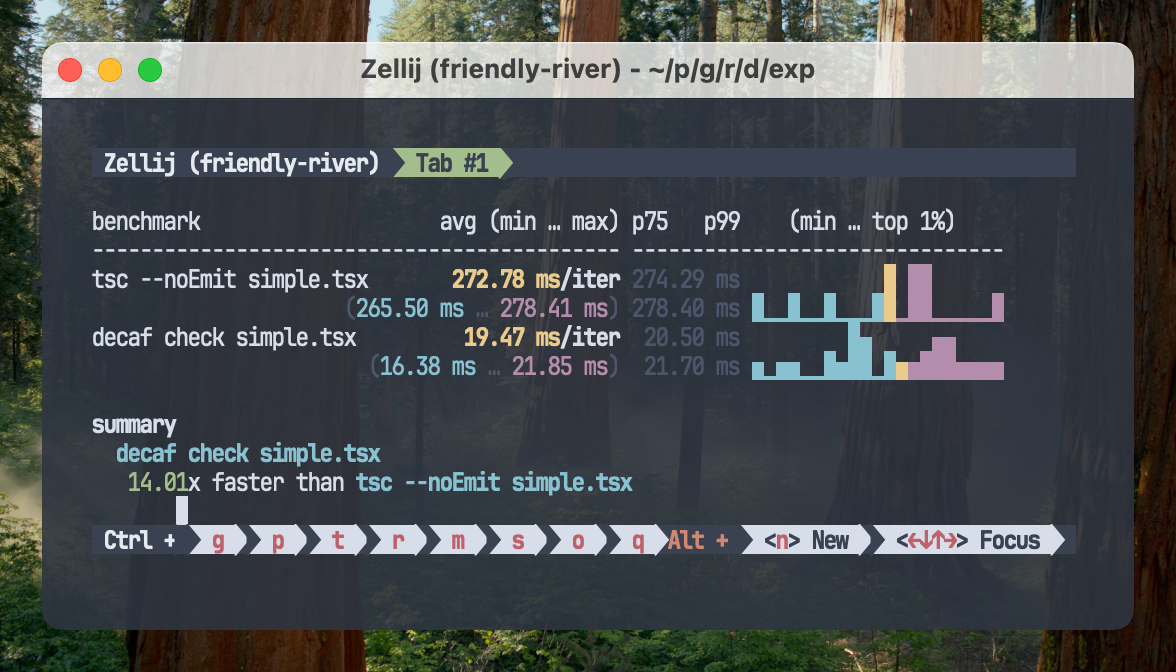
\includegraphics[width=0.8\textwidth]{figures/fig_exp_1_simple_tsx.png}
    \caption{\texttt{simple.tsx} を decaf と tsc で型検査した結果}
    \label{fig:simple}
\end{figure}

ベンチマーク結果を見ると, decaf は tsc の 14.01 倍の速度で型検査をしていることがわかる.

\subsection{middle.tsx}

\ref{fig:middle}に\texttt{middle.tsx}を decaf と tsc で型検査した結果を示す.

\begin{figure}[H]
    \centering
    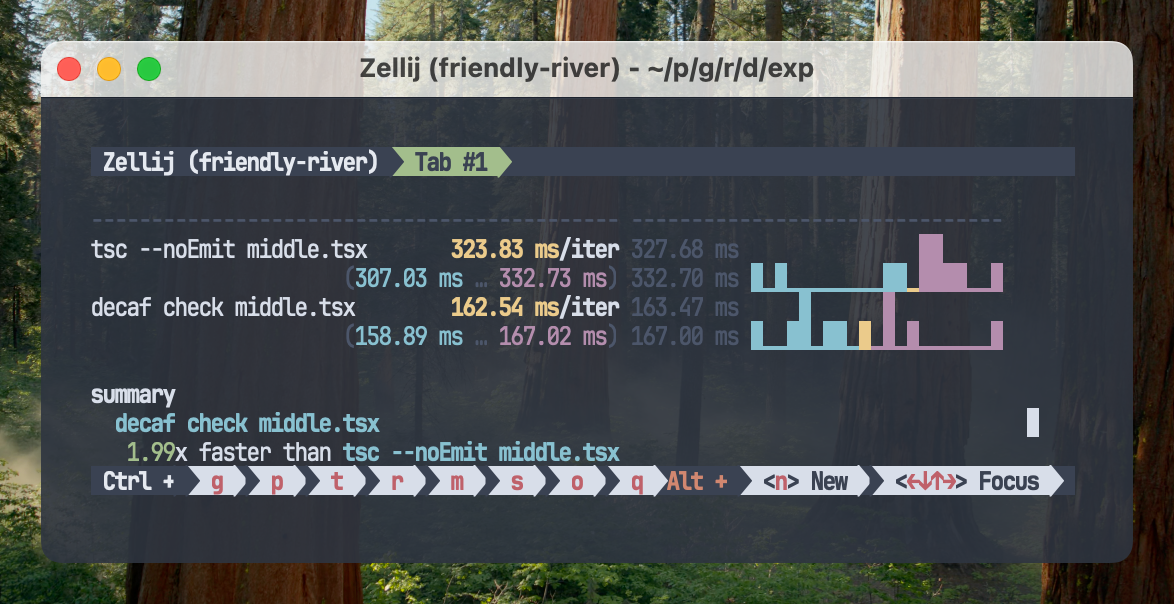
\includegraphics[width=0.8\textwidth]{figures/fig_exp_1_middle_tsx.png}
    \caption{\texttt{middle.tsx} を decaf と tsc で型検査した結果}
    \label{fig:middle}
\end{figure}

ベンチマーク結果を見ると,decaf は tsc の 1.99 倍の速度で型検査をしていることがわかる.

\subsection{complex.tsx}

\ref{fig:complex}に\texttt{complex.tsx}を decaf と tsc で型検査した結果を示す.

\begin{figure}[H]
    \centering
    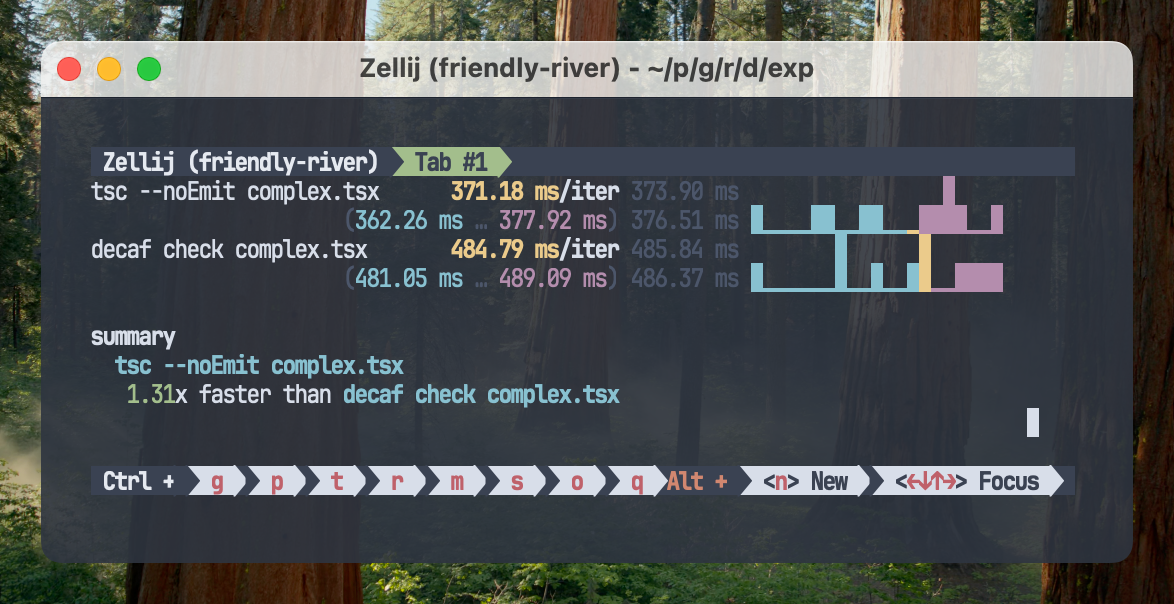
\includegraphics[width=0.8\textwidth]{figures/fig_exp_1_complex_tsx.png}
    \caption{\texttt{complex.tsx} を decaf と tsc で型検査した結果}
    \label{fig:complex}
\end{figure}

ベンチマーク結果を見ると, tsc は decaf の 1.31 倍の速度で型検査をしていることがわかる.

\subsection{very\_complex.tsx}

\ref{fig:very_complex}に\texttt{very\_complex.tsx}を decaf と tsc で型検査した結果を示す.

\begin{figure}[H]
    \centering
    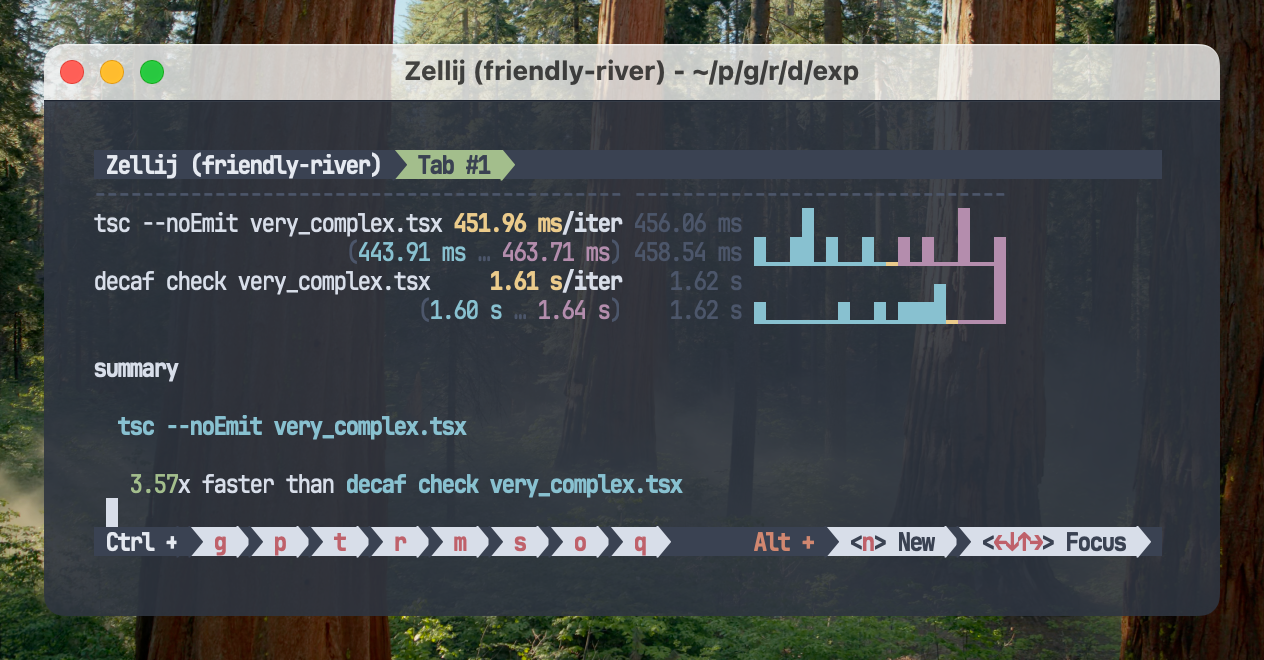
\includegraphics[width=0.8\textwidth]{figures/fig_exp_1_very_complex_tsx.png}
    \caption{\texttt{very\_complex.tsx} を decaf と tsc で型検査した結果}
    \label{fig:very_complex}
\end{figure}

ベンチマーク結果を見ると, tsc は decaf の 3.57 倍の速度で型検査をしていることがわかる.

\section{考察}
\label{sec:consideration}

各ベンチマークにおいて,常に decaf が tsc よりも速い結果とはならなかった.
そこで,型検査機ごとのベンチマークケースごとの速度を棒グラフにしたものが以下である.

\begin{figure}[H]
    \centering
    \begin{minipage}[b]{0.49\columnwidth}
        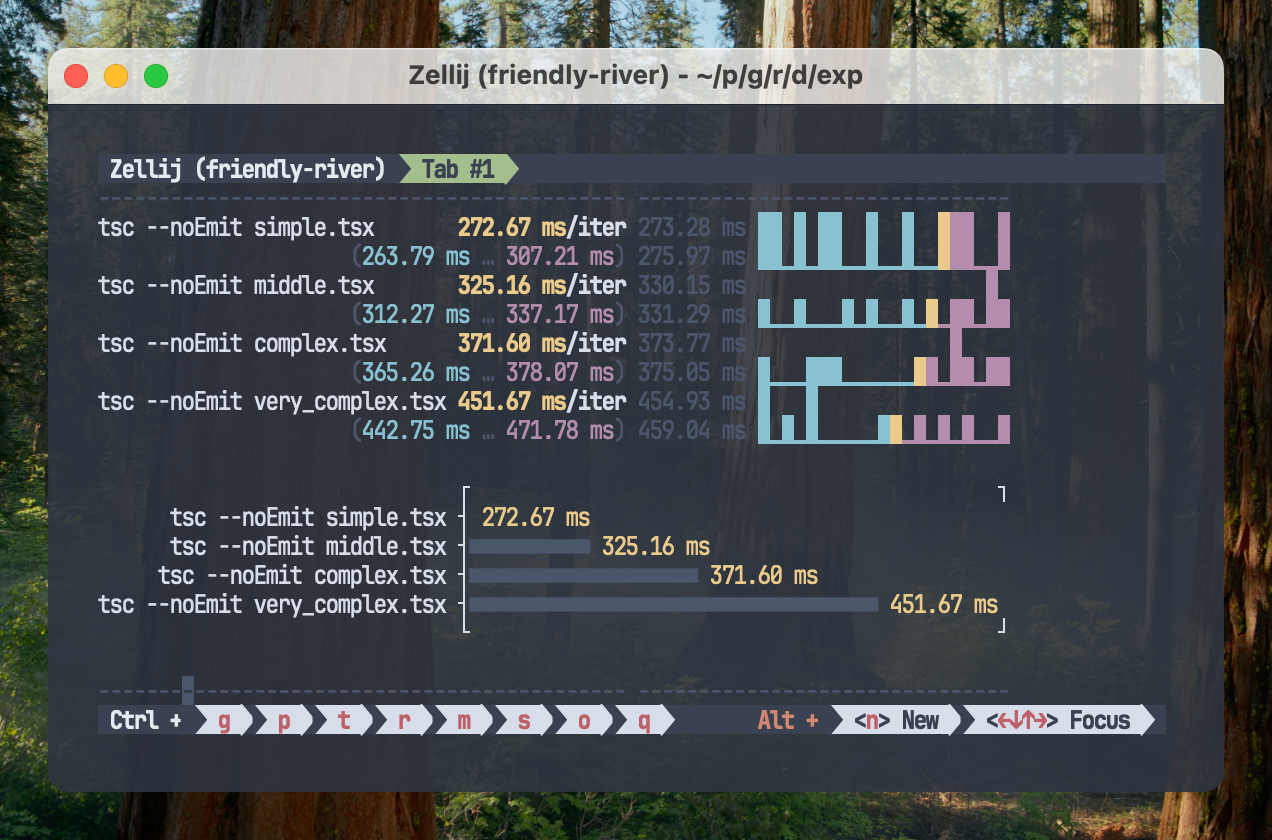
\includegraphics[width=\columnwidth]{figures/fig_exp_1_tsc_barplot.png}
        \caption{tsc の型検査速度}
        \label{fig:barplot_tsc}
    \end{minipage}
    \begin{minipage}[b]{0.49\columnwidth}
        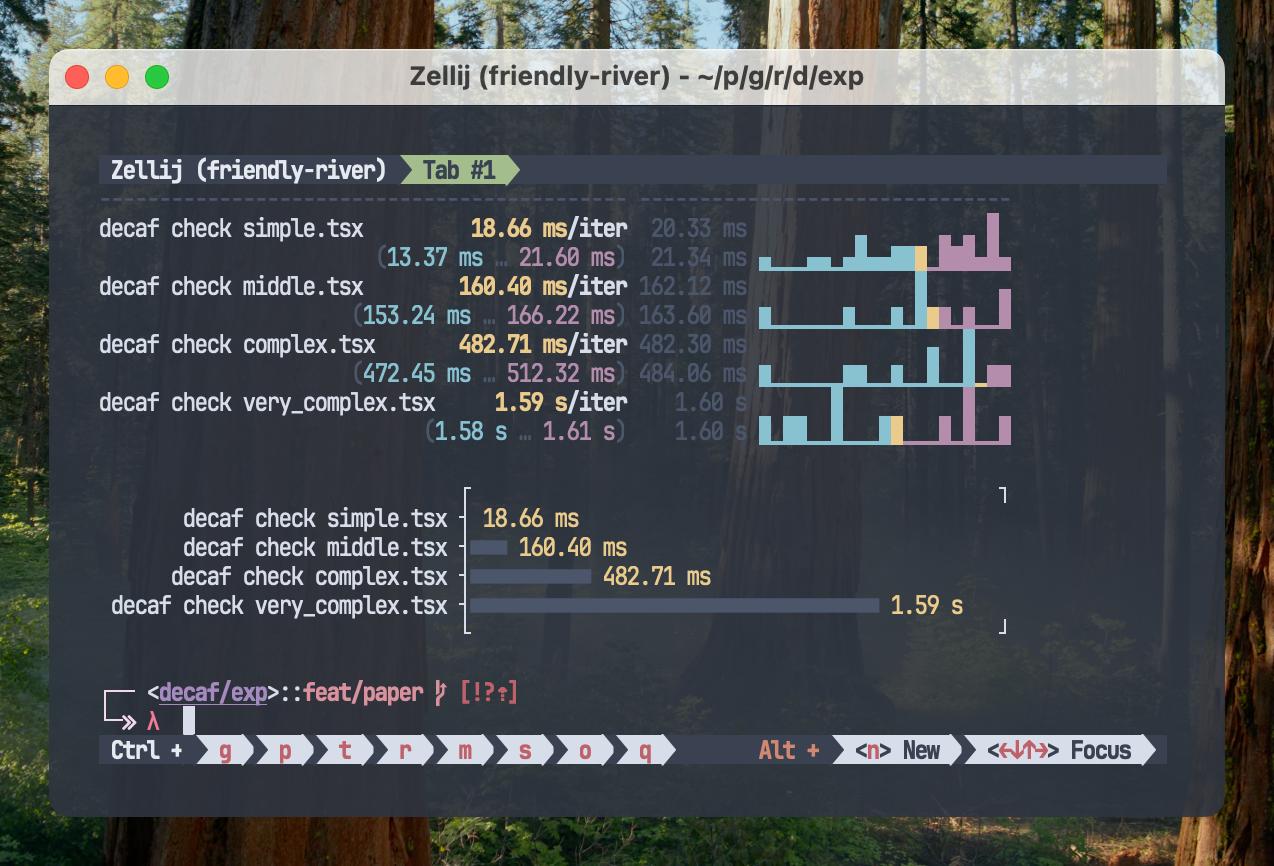
\includegraphics[width=\columnwidth]{figures/fig_exp_1_decaf_barplot.png}
        \caption{decaf の型検査速度}
        \label{fig:barplot_decaf}
    \end{minipage}
\end{figure}

\ref{fig:barplot_tsc}を見ると,ベンチマークケースごとの速度の平均が,272.67ms 〜 451.67ms の範囲にある.
対して,\ref{fig:barplot_decaf}を見ると,ベンチマークケースごとの速度の平均が, 18.66ms 〜 1,590.00ms の範囲にある.
結果として,プログラムのサイズが大きくなると decaf の型検査速度は遅くなることがわかった.

これは,decaf が tsc と比べてより多くの情報をプログラムから抽出し,より厳格な型システムを表現しているからだと考える.
\ref{fig:barplot_tsc}の数値の推移を見ると,プログラムの規模を$n$としたとき,$O(n)$の時間で型検査していることがわかる($y = 4.52n + 275$, $R^2 = 0.993$).
一方で,\ref{fig:barplot_decaf}の数値の推移を見ると,プログラムの規模を$n$としたとき,$O(n^2)$の時間で型検査していることがわかる($y = 0.799n^2 + 7.58n + 8.68$, $R^2 = 1.00$).
回帰式から decaf の型検査速度は tsc よりも遅い場合があるが,それは decaf の型検査速度はプログラムのサイズに対してより高次の計算量を持つことが原因である.
これは,それぞれの型検査機のアルゴリズムによるものである.
\ref{sec:decaf-check}で述べた通り,decaf は tsc よりも多くの経路を型検査するため,より厳格な型システムを実現している.
そのため,decaf は tsc と比較したときに巨大なプログラムに対しては遅いという結果になった.

一方で,\ref{sec:simple}のような標準的なケースにおいて,decaf は tsc よりも速い結果となった.
これは若干の結果論を含むが,\ref{sec:simple}のケースだけでもソースコードの長さは,2949 行もある.
基本的にこの行数のコードが 1 つのファイルに書かれるのは技術負債として避けるべきである.
そのため,decaf は tsc と比べてより厳格な型システムを実現しているが,標準的なケースにおいては tsc よりも速い結果となったと言えるだろう.
また,回帰式の y 切片はそれぞれのコンパイラの初期化時間を表しており,decaf は tsc よりも初期化時間が短いことがわかる.
decaf や tsc はその機能が Language Server や Linter にも使うことができるため,初期化時間が短いことはユーザビリティにも影響を与える.

\section{decafの改善点}

まず,現在の TypeScript がサポートしている構文\footnote{執筆時点での最新バージョンは\href{https://github.com/microsoft/TypeScript/tree/v5.7.3}{v5.7.3}である}の全てに対応していない.
そのいくつかは decaf の型の厳密性を実現するために実装をしないと決めているものもある.
しかし,decaf の内部実装や仕様を熟知していないと,decaf の型検査が通らない理由は分からない.
そのためより多くの構文をサポートすると同時に,分かりやすいエラー形式を提供することが望ましい.

また,\ref{sec:decaf-check}で述べた通り,decaf は tsc よりも多くの経路を型検査するため,大きなプログラムに対しては遅いという問題がある.
decaf の型検査に用いられる TypeID は,不可分であり本来はパースを並列で行える.
だが,現在の実装ではパースを逐次で行っているため,TypeID の生成に時間がかかっている.
そのため,TypeID の生成を並列で行うことで,decaf の型検査速度を向上させることができるだろう.
